\documentclass[12pt]{jpconf}
%\documentclass[10pt, landscape, twocolumn]{article}

\usepackage{graphicx}
\usepackage{amsmath, amssymb}

\usepackage{xcolor}
\definecolor{amaranth}{rgb}{0.9, 0.17, 0.31}
\definecolor{amethyst}{rgb}{0.6, 0.4, 0.8}
\definecolor{ao}{rgb}{0.0, 0.0, 1.0}



\begin {document}
\title{Application of convolutional neural networks in optical text recognition to junk data filtering}
\author{Razumov T.E., Churikov D.V., Kravchenko O.V.}

\address{Production Editor, \jpcs, \iopp, Dirac House, Temple Back, Bristol BS1~6BE, UK}

\ead{jacky.mucklow@iop.org}


\begin{abstract}
	In this paper, the problem of constructing a model for detecting and filtering unwanted spam messages is solved. A fully connected convolutional neural network (\textsf{FCNN}) was chosen as the model of the classifier of unwanted emails in email. It allows you to divide emails into two categories: \emph{spam} and \emph{not spam}.
	The main result of the research is a software application in the \textsf{C++} language, which has a micro-service architecture, and solves the problem of image classification. The app is able to handle more than $10 ^ 6 $ requests per minute in real time.
\end{abstract}

% --------------------
\section{Introduction}
Presently, the amount of information produced by humanity
is growing exponentially. Significant benefits can be derived from this information only if the data is properly processed and analyzed.
On the other hand, the actual task of data processing in general is the task of junk data filtering and it transforms into the task of spam messages filtering in case of IT technologies particularly.
The latter is due to the fact that the exchange of information of various information by default uses email. It's one of the cheapest, easiest to use, most easily accessible, official, and most reliable way to communicaty nowadays.
Junk data or spam messages, generally speaking, may contain heterogeneous test--visual information. Modern deep
learning algorithms are used to analyze emails traffic with various information received in real time \cite{Makkar2021}.
In this case, first features (characteristics) are extracted from the image, and then a decision is made.
Another approach is a classification one that include the support vector machine algorithm and the random forest method. These methods for solving the problem of filtering spam messages are compared in \cite{Taylor2020}.
At the same time, filtering algorithms are usually stochastic \cite{Garg2021} and are used in combination with optimization techniques for some objective function. Various probabilistic models are used to solve the problem of email classification. One of the most commonly used approach is the naive Bayesian classifier. Other one is the particle swarm method is one of the numerical methods of stochastic optimization and it is used in data filtering problems, since it is not necessary to specify an analytical expression of the gradient of the optimized function. The particle swarm method refers to stochastic optimization methods and it is utilized for heuristic global optimization of the parameters of a naive Bayesian classifier. A complex approach using the naive Bayes algorithm together with the particle swarm optimization method was applied in \cite{Parmar2020}.
The evolutionary model of spam classification is also presented in \cite{Mohammad2020}.

The problem of detecting and filtering unwanted spam messages is investigated in present paper. A fully connected convolutional neural network (\textsf{FCNN}) is considered as a solution tool, which was chosen to classify junk email messages.


\section{Methodology}
\subsection{Statement of the problem}
Let's consider a set of objects $ X = X_L \cup X_T$, where
$X_L$ is training sample,
$X_T$ is test sample,
$Y$ is set of valid responses. Also, assume that there is an objective function $g: X \rightarrow Y$, whose values are known only on the set $X_L$. Let the data be distributed according to some unknown distribution $P (x,y) = P(x) P (y|x)$, with some loss function given
$$
R(g(x), y) = 
\begin{cases} 
\phantom{>}0, & y = g(x), \\
> 0, & y \neq g(x).
\end{cases}
$$
In accordance with the principle of minimizing empirical risk, the loss function is used to be minimazied. In other words a decision function $g(x)$, which on average will lead to the smallest error is determined. Formally, one need to solve the minimization problem as follows
$$
g(x) = \operatorname*{argmin}_{f: X \rightarrow Y} E_{X,Y} R(f(x), y).
$$
To state the problem of junk data filtration, the set $Y$ consists of two elements $\{0, 1\}$, where $0$ and $1$ are desirable and undesirable data, respectively. Due to the roughness of the discrete computing methods $R = P[0, 1]$ is usually used in practice. Thus,the result of the classifier $r' = r(x)$ belongs to the desired class with a given threshold probability $\alpha$, which minimizes the error of the first and second kind.

\subsection{Requirements for the solution}
Since, the speed of the information traffic increases an additional important requirement on the speed of the model and the system as a whole is imposed. The time for checking a single message should not exceed $\leqslant3$ seconds, which imposes additional constraint on the tools utilized and on the fault tolerance of the entire system.
From the moment of receiving the message to the moment of making a decision about its type the text information goes through three stages of processing, such as
\begin{itemize}
\item Preprocessing.
\item Vectorization.
\item Classification.
\end{itemize}

\subsection{Text preprocessing}
Since the text has a very heterogeneous structure and a single word can be written in many different ways (different font, encoding, case, etc.), but still have the same meaning, different methods of preprocessing the text or a combination of them are used.
The first step is to parse the text and decode it into the specified encoding. Then the conversion to the lower (or upper) case, removing unnecessary spaces, indents. The characters are replaced according to the specified rule. After that, the following methods are applied:

\subsubsection*{\it\,Stop words}
The text often contains many characters that do not carry a semantic load for the general meaning (two spaces, paragraph indentation), as well as stop words.
Stop words are words in any language that don't add much meaning to a sentence. Often, stop words include punctuation marks, pronouns, and prepositions. Often, spammers use them to make texts noisy in order to hide the spam content of the message. Since they can be safely ignored without sacrificing the meaning of the sentence, classification tasks often resort to removing them from the original message.

\subsubsection{\it\,Stemming and lemmatization}
Usually texts contain different grammatical forms of the same word, and may also contain the same root words. Using different algorithms, lemmatization and stemming aim to reduce all occurring word forms to a single, normal dictionary form.


Stemming is a crude heuristic process which cuts off "extra" from the word root, often resulting in a loss of word-formation suffixes. The main problem encountered when using stemming is the processing of words which, when forming different grammatical forms, change not only the ending, but also the base of the word. For example, the noun "cat" in the accusative and genitive plural has the form "cats. Because of such fluent vowels, a streamer must either ignore such forms, truncating "cats" to "koshk" and losing some of the word forms, or truncate the word to an unchangeable stem, obtaining "kosh," which can then lead to a complete loss of context. To minimize the negative consequences of too aggressive truncation of words by the streamer, it is necessary to perform memming of the searched keyword, and then compare the result with the output of the streamer for each of the words in the processed text. Even so, you will come across stems for entirely unrelated words.


Lemmatization is a more subtle process, which uses dictionary and morphological analysis to reduce a word to its canonical form (lemma). However, it applies simplistic word analysis without considering the context. This leads to ambiguities in determining parts of speech. For example, the lemmatization of the words in the phrase "we dig a hole" will yield two lemmatization options for the second word: the noun swarm and the verb dig. This ambiguity cannot be resolved without involving the morphological analyzer.

As a rule, lemmatization gives the most accurate results, and this is the approach used in the work.

\subsection{Text vectorization}
Modern machine learning algorithms cannot directly work with raw text, so it is necessary to build a text mapping to a vector space. This is called feature extraction. Let's consider several approaches for constructing this mapping.

\subsubsection{\it\,Bag of words}
The "bag of words" model is a simplified representation of textual information used in natural language processing and information retrieval tasks. In this model, the text is represented as a bag (multiset) of its words or phrases in the case of combinations of terms, ignoring grammar and in some cases even word order, but preserving multiplicity. Each such term (word or phrase) is assigned a number. In this case, the text is defined by the vector $x=(x_1,..., x_N)^T$, where $N$ is the dimension from the finite dictionary $X_L$ consisting of unique terms of the training sample. The following options for defining $x_i$ are possible
\begin{itemize}
\item Boolean weight equals $1,$ if element exists in a message or 
$0,$ else.
\item The number of occurrences of the $i$--th term in the text is 
$x_i = n_i.$
\item Term frequency is $x_i = n_i\left(\sum\limits_{k=1}^i n_k\right)^{-1}.$
\end{itemize}
To determine $x_i$, the frequency of the term is selected.

\subsubsection{Word2Vec}
The main problem with BOW is the loss of context between words. Since in natural language, the permutation of even two words of a sentence can completely change its meaning, this classification approach may have low accuracy.

Word2Vec is a text vectorization tool that takes into account the contextual relationship between words. The algorithm is based on such methods as huffman binary tree, skip-gram, negative sampling. The main problem with Word2Vec is finding the context for rare words.

\subsubsection{Fast Text}
FastText is a Word2Vec extension proposed by Facebook in 2016. Instead of entering individual words into a neural network, Fast Text splits the words into several n-grams (proverbs). For example, the trigrams for the word "apple" --- are "app", "ppl", and "pll" (excluding the beginning and end of word boundaries). The vector for the word "apple" is formed by the sum of all n-grams. After training the neural network, we will have embedding words for all n-grams from the training dataset.
With this approach, the algorithm becomes more sensitive to rare words, since it is very likely that some of their n-grams are also present in other words. It takes longer to train the Fastext model, but it works better than Word2Vec and allows you to correctly represent rare words.

\subsection{Text classification}
After vectorizing the text, we must construct a transformation from a set of features to a set of classifiable objects $g: X \rightarrow Y.$
According to the article [twitter threshold p. 4.6], unique points were marked by bins and the optimal threshold accuracy $ \ alpha = 0.75$ was calculated, which provides optimal pressision and recall for our model and minimizes the error variance.

\subsubsection{Logistic regression}
The commonly used approach in the classification is the logistic regression method
$$
g(x) = \left(1 + \exp{ \left( \sum_{i=0}^n w_i x_i  \right) }\right)^{-1},
$$
where $\mathbf{w}=(w_1,\ldots, w_N)^T$ is weights of the model are obtained during training.
Here are the results of calculations for different methods of text vectorization.
The results for BOW and Fast Text embeddings, are introduced in table\,\ref{tbl:01}.
\begin{table}
	\centering
	\caption{\label{tbl:01}Training result.}
	\begin{center}
		\begin{tabular}{lll}
			\br
			embeddings & precision & recall \\
			\mr
			BOW & 0.91143 & 0.99961 \\ \hline
			Fast Text & \bf 0.95523 & \bf 0.89164 \\ 
			\br
		\end{tabular}
	\end{center}
\end{table}

\subsubsection{Fully convolutional neural network}
The fully convolutional neural network with 3 layers was considered. The first two use the \textsf{ReLU} activation function, and the last one uses \textsf{sigmoid}. Data is regularized on each layer. In our case, the neural network can be defined by the formula
$$
g(x) = h_2 \left(\sum_{k=0}^{n_2} w''_k h_1\left(\sum_{j=0}^{n_1} w'_j h_0\left( \sum_{i=0}^{n_0} w_i x_i \right)\right)\right),
$$
where $h_i$ is the activation function for the corresponding layer. To find the weights $\{w_i\}$, $\{w'_j\}$, $\{w''_k\}$ at the model training stage, the Adam method is used.
The results for BOW and Fast Text embeddings, are also introduced in table\,\ref{tbl:02}.
\begin{table}
	\centering
	\caption{\label{tbl:02}Training result.}
	\begin{center}
	\begin{tabular}{lll}
		\br
		embeddings & precision & recall \\
		\mr
		BOW & 0.93604 & 0.95643 \\ \hline
		Fast Text & \bf 0.99931 & \bf 0.91263 \\ 
		\br
	\end{tabular}
	\end{center}
\end{table}

\subsection{Aspects of algorithm implementation}
\subsubsection{Microservice architecture}
Since the service must operate under high loads, it is important to provide an architecture in which the failure of one component does not lead to the degradation of the entire system. The following client-server architecture is implemented (Fig. 1). Antispam daemon (mrasd) parses incoming messages and extracts text, images, and files from there. Since unwanted data is often contained inside nested images and documents, it is also necessary to extract text from them. To do this, the documents are sent to the OCR service via a deferred redis queue, which extracts the text and stores the result in the redis cache.

\begin{figure}[t]
	\center
	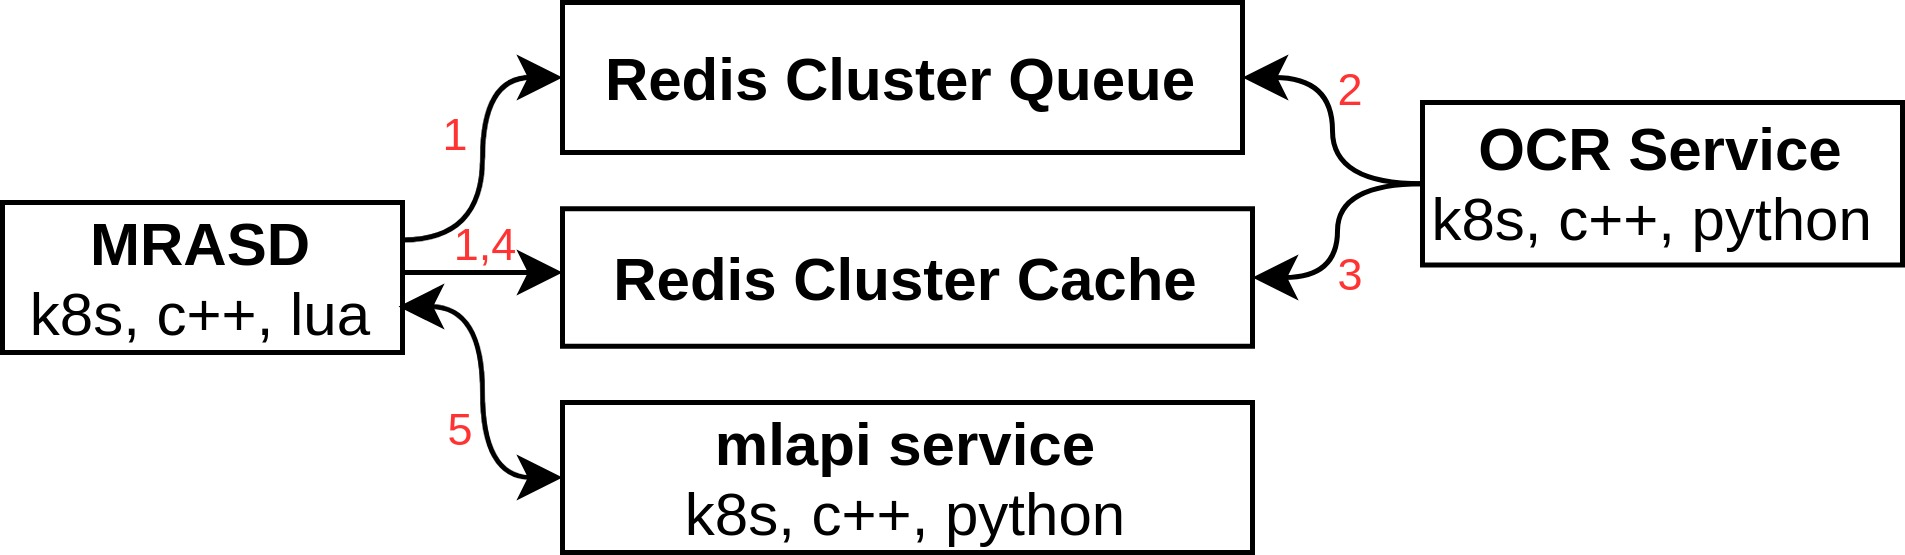
\includegraphics[width=0.95\textwidth]{images/deploy.jpg}
	\caption{\label{fig:02} Deploy}
\end{figure}

\begin{figure}[b]
	\center
	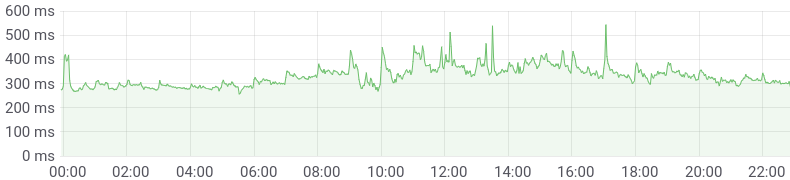
\includegraphics[width=0.95\textwidth]{images/timings.png}
	\caption{\label{fig:03} Average email processing time}	
\end{figure}


Since, with a high probability, the letter can be a duplicate (for example, in the case of a ddos attack or offline rechecking), in order not to load the OCR service once again, the primary check of the redis cache is performed for the presence of already processed data for the specified document hash.

After full text extraction, the mrasd service performs all the steps of text preprocessing (reduction to a single register, removal of stop words, normalization), and then sends the text to the mlapi service via the grpc protocol to vectorize the text using fast text and further obtain the fcnn prediction of the model by which a decision is made about the" undesirability " of the incoming message.

The proposed architecture is good because when the OCR of seris, one (or several) instances of redis cluster fails, the entire system as a whole does not degrade.
 
\begin{figure}[t]
	\center
	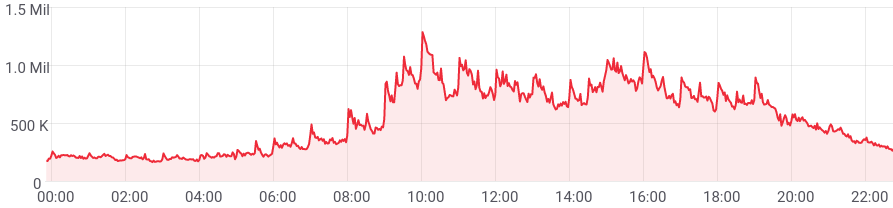
\includegraphics[width=0.95\textwidth]{images/processed_messages.png}
	\caption{\label{fig:04} Average number of requests per minute from one of the farms}
\end{figure}

\subsubsection{Brief review of the libraries}

Since services require high performance, the C++ language (stl 17, grpc, boost) is chosen for writing it, as one of the most productive modern languages. For data analysis and training of the AST model, the Python 3 language and the utouch framework were used due to the high efficiency and the possibility of conducting parallel calculations, both on the CPU and on the GPU cores of the machine.

The fault tolerance of microservices is ensured by their deployment in the kubernetes (k8s) cluster, since if any pod falls for any reason, the requests are evenly balanced across the remaining live feeds, until the cluster independently returns to its previous state. Inside it, you can configure: automatic load balancing by constantly monitoring information about performance and resources used (autoscaling) and competent placement of hearths within the cluster by data centers (affinity).

\section{Conclusions}

The results obtained during the training of the model on real streaming data of users are introduced. Based on these data, one can realize that \textsf{FCNN} model based on Fast Text embeddings has higher classification accuracy rather then method of classical logistic regression and \textsf{FCNN}  model based on a bag of words.


A high--performance fault--tolerant microservice architecture is presented, which can withstand an average of more than $10^6$  requests per minute. At the same time, the degradation of a specific component, machine, or data center does not lead to complete inactivity of the application.

\section*{References}
\begin{thebibliography}{99}
\bibitem{Makkar2021} 
Aaisha Makkar, Uttam Ghosh, Pradip Kumar Sharma.
2021. \emph{Artificial Intelligence and Edge Computing-enabled
	Web Spam Detection for Next Generation IoT
	Applications} // IEEE Sensors Journal

\bibitem{Taylor2020}
Taylor O.E., Ezekiel P.S.
2020. \emph{A Model to Detect Spam Email Using Support Vector Classifier and Random Forest Classifier} //
International Journal of Computer Science and Mathematical Theory

\bibitem{Garg2021}
Pranjul Garg, Nancy Girdhar.
2021. \emph{A systematic review on spam filtering techniques based on
natural language processing framework} // 2021 11th International Conference on Cloud Computing, Data Science \& Engineering (Confluence 2021)

\bibitem{Parmar2020}
Nandan Parmar, Ankita Sharma, Harshita Jain, Amol K. Kadam.
2020. \emph{Email Spam Detection using Naïve Bayes and Particle Swarm Optimization} // IJIRT

\bibitem{Mohammad2020}
Rami Mustafa A. Mohammad.
2020. \emph{A lifelong spam emails 	classification model} //
Applied Computing and Informatics
\end{thebibliography}



\end {document}
